\chapter{Implementierung}
\label{ch:implementierung}
Das Kapitel Implementierung erfasst die technische Dokumentation des erarbeiteten Prototyps.
Im Detail werden in den folgenden Seiten die technische Umsetzung des in Kapitel \ref{ch:concept} entworfenen Konzepts beschrieben. 
Beschriebene Funktionalitäten werden mit Bildausschnitten unterstützt.

\section{Prototyp}
Die Anwendung wurde als Angular Projekt mittels der Angular CLI erstellt. 
Über den CLI Befehl 

\begin{lstlisting}[language=bash]
$ ng new gravitationsmodel
\end{lstlisting}

generiert die CLI ein kompilierbares und ausführbares Angular Projekt mit essentiellen Abhängigkeiten und Strukturen.
Angular verwendet standardmäßig NPM als package manager.
Eine \emph{package.json}, welche sämtliche Abhängigkeiten dokumentiert, wird bereits mit erstellt.
Um das Setup abzuschließen müssen weitere Abhängigkeiten in Form von \emph{npm packages} installiert werden.
Über den Befehl 

\begin{lstlisting}[language=bash]
$ ng add ol
\end{lstlisting}

fügt die CLI automatisch das Paket von OpenLayers hinzu und für die korrekte Typisierung in TypeScript das notwendige \emph{types} Paket für OpenLayers hinzu.

Nachdem die technischen Voraussetzungen geschaffen sind kann mit der Implementierung begonnen werden.
Auch hierbei bietet die CLI Unterstützung in Form von \emph{Scaffolding} Befehlen.

\begin{lstlisting}[language=bash]
$ ng generate <schematic> [name]
\end{lstlisting}

generiert Komponenten, Services, Models, Klassen und weitere Code-Gerüste durch den passenden Präfix-Parameter und Namen.
Angular Komponenten bestehen meist aus einer TypeScript-Klasse (\emph{.component.ts}), einem Template (\emph{.component.html}) sowie Dateien für Styling (\emph{.css} oder \emph{.scss}) und Tests (\emph{.component.spec.ts}).

\begin{lstlisting}[language=bash]
$ ng generate component objektfenster
\end{lstlisting}

erstellt \emph{objektfenster.component.ts}, \emph{objektfenster.component.html} sowie \emph{objektfenster.scss} und \emph{objektfenster.component.spec.ts} Dateien.

Mit Hilfe der CLI lassen sich so die Code-Gerüste schnell erstellen und die CLI übernimmt sogar die in Angular nötige \emph{Dependency Injection} indem neue Komponenten direkt in der entsprechenden \emph{.module.ts} deklariert werden \footcite{angular_cli}.

Ebenfalls im Zuge der Projekterstellung über die CLI werden Konfigurationsdateien angelegt, die wichtige Einstellungen zum Kompilieren, Bau, Start und Hosten (engl. host) der Anwendung enthalten.

Die Anwendung kann nun über 

\begin{lstlisting}[language=bash]
	$ ng serve
\end{lstlisting}

gestartet werden.
Der Befehl kompiliert, baut und startet die Anwendung über einen lokalen Webserver.
Über \emph{localhost:4200} kann die Anwendung im Browser aufgerufen werden.

Der Kern der Anwendung ist eine Karte mit der interagiert wird.
Um diese darzustellen, muss zunächst ein OpenLayers Map-Objekt erstellt und in den DOM eingehängt werden \footcite{openlayers_map}.
Dies geschieht in der OpenLayersMap-Komponente und dem BaseMap-Service.
Über das bereits installierte OpenLayers Paket wird das Map-Objekt importiert und initialisiert.

\begin{lstlisting}[language=JavaScript]

	const targetId = 'map';
	const longitude = 13.451338;
	const latitude = 52.503707;
	const zoomLevel = 11;
	
	const coordinate = fromLonLat([longitude, latitude]);
	
	const view = new View({
		center: coordinate,
		zoom: zoomLevel
	});
	
	const map = new Map({
		target: targetId,
		layers: [],
		view,
	});


\end{lstlisting}

Die Karte wird mit der notwendigen Id des HTML-Elements, in welchem die Karte angezeigt werden soll, und einem View initialisiert.
Das View-Objekt besteht aus einer Center-Koordinate und der initialen Zoomstufe und stellt den Begrenzungsrahmen (engl. Bounding Box) der Karte dar.
Zu beachten ist ebenfalls hierbei die Transformation der Koordinaten von EPSG:4326 in das in OpenLayers standardmäßig genutzte EPSG:3857 über die Funktion \emph{fromLonLat}.
Die Karte wird ebenfalls mit Standard-Interactions und Standard-Controls initialisiert jedoch sind noch keine Layer hinzugefügt.
Somit ist jetzt auch noch nichts auf der Karte zu sehen und lediglich bereits erwähnte Controls und Interactions sind sichtbar und bedienbar.
Hierzu zählen:

\begin{itemize}[Controls]
	\item Zoom
	\item Rotate (Unsichtbar bei Rotation 0)
	\item Attribution
\end{itemize}

\begin{itemize}[Interactions]
	\item Drag rotate
	\item Drag pan
	\item Drag zoom
	\item Double click zoom
	\item Mouse wheel zoom
	\item Pinch rotate (Touchscreen)
	\item Pinch zoom (Touchscreen)
	\item Keyboard pan
	\item Keyboard zoom
\end{itemize}

Als nächstes wird der Hintergrundkarten-Layer hinzugefügt.
Hierzu wird ein neuer Tilelayer initialisiert, eine neue Layer-Quelle (engl. Source) hinzugefügt und der Layer der Karte hinzugefügt.

\begin{lstlisting}[language=JavaScript]
	
	const backgroundLayer = new TileLayer();
	backgroundLayer.setSource(new OSM());
	backgroundLayer.set('name', 'Hintergrund');
	
	map.addLayer(backgroundLayer);	
	
\end{lstlisting}

Der Hintergrundkarten-Layer ist ein Kachel (engl. Tile) Layer, da dies die Datenabfrage an den Kartendienstleister, in diesem Fall OpenStreetMaps, reduziert und eine optimale Render-Performance erzeugt.
Ein Tile-Layer teilt den Kartenausschnitt in ein Gitter (engl. Grid) aus vielen kleinen Kacheln ein.
Jeder dieser Kacheln setzt ihren eigenen Http-Request an den in der Source angegeben Provider mit den Kachel-Koordinaten und Zoom-Stufe als Parameter ab und bekommt einen Kartenausschnitt in PNG-Format zurück.
Die einzelnen Bilder werden dann im Cache des Browsers gespeichert und sorgen somit für verminderten Datentransfer sowie schnelles Laden bei erneutem Aufruf.
OpenLayers bietet für OpenStreetMap sowie Bing Maps eigene Source-Objekte, welche für Bing nur noch einen API-Key benötigt.
Um den Layer später einmal einfach identifizieren zu können, wird dem Layer noch eine Name-Eigenschaft zugewiesen.

Nach der Hintergrundkarte müssen nun noch Layer für die Filialen sowie die Zensusgebiete implementiert werden.
In der OpenLayersMap-Komponente werden dazu zwei neue Layer mit passenden Source-Objekten angelegt.

\begin{lstlisting}[language=JavaScript]

	const filialLayer = new VectorImageLayer({
		visible: true,
		zIndex: 2
	});	
	filialLayer.set('name', 'Filialen');
	filialLayer.setSource = new VectorSource({
		format: this.geoJSONFormat,
		strategy: bbox	
	});

	const gebieteLayer = new VectorImageLayer({
		visible: true,
		zIndex: 1
	});
	gebieteLayer.set('name', 'Gebiete');
	gebieteLayer.setSource = new VectorSource({
		format: this.geoJSONFormat,
		strategy: bbox	
	});

	map.addLayer(filialLayer);
	map.addLayer(gebieteLayer);
\end{lstlisting}

Bei der Initialisierung der Layer muss die Z-Ebene der Filialen höher sein, da sie später in der Anwendung über den Gebieten liegen sollen und nicht von diesen überlagert werden sollen.
Bei VectorSources kann zwischen den Ladestrategien Tile und Bounding Box entschieden werden.
Sie bestimmt wann neue Features auf der Karte geladen und angezeigt werden sollen.
Bei der Tile-Strategie wird wie bei der Hintergrundkarte der Kartenausschnitt in ein Kachelgitter unterteilt und bei der Bounding Box Strategie wird der gesamte Kartenausschnitt (engl. Bounding Box) gewählt. 
Bei besonders vielen Daten sollte auf die Tile-Strategie zurückgegriffen werden aber im Prototypen reicht die Bounding Box Strategie vollkommen aus.

OpenLayers definiert standardmäßig für jeden Vector Layer einen Stil, der die einzelnen Features je nach Geometrietyp auf der Karte darstellt. 
Soll dieser Stil geändert werden, muss auf dem Layer ein neuer Stil definiert werden.
Dies kann über ein statisches Style-Objekt erfolgen oder über eine dynamische Style-Funktion.

\begin{lstlisting}[language=JavaScript, label={code:filialStyle}]
	
	const filialStyle = new Style({
		image: new Icon({
			color: '673ab7'
		}),
		text: new Text({
			fill: new Fill({
				color: 'FFFFFF'
			})	
		})
	});
	
	const filialStyleFunction = (feature, resolution) => {
		if (feature.get('selected') === true) {
			filialStyle.getImage()
			.setSource('assets/geometries/icons/PIN_selected.svg');
		} else {
			filialStyle.getImage()
			.setSource('assets/geometries/icons/PIN.svg');
		}
		filialStyle.getText().setText(feature.getId().toString());
		return filialStyle;
	}
	
	filialLayer.setStyle(filialStyleFunction);

	
\end{lstlisting}

Nun werden realistische Geo- sowie Marktdaten benötigt.\\
Die Filialen sind einfache Koordinaten im Raum Berlin.
Ein Testdatensatz mit 97 Koordinaten wurde über geojson.io \footnote{\href{geojson.io}{geojson.io}} angelegt.
Die Koordinatenliste wird bereits in GeoJSON angelegt und die Einträge müssen lediglich um eine Id, Anzahl der Parkplätze sowie die Verkaufsfläche der Filiale ergänzt werden.\\
Ein Testdatensatz mit 1220 Zensusgebieten des Geoportals Berlin \footcite{geoportal_berlin} wurde über das ArcGIS Hub \footcite{arcgis_verkehrszellen} heruntergeladen.
Die Gebiete werden ebenfalls bereits in GeoJSON exportiert.
Da es sich jedoch um zu viele Einträge für eine manuelle Ergänzung der Marktdaten handelt, werden Marktdaten für die einzelnen Gebiete beim einlesen der Datei ergänzt.

Die Datensätze werden über das Feature Format GeoJSON in OpenLayers eingelesen und in eine FeatureCollection (bei einzelnen Daten in ein Feature) umgewandelt, welche der jeweiligen Layer Source hinzugefügt wird.

\begin{lstlisting}[language=JavaScript]

		this.http.get('../assets/filialen.json').subscribe(value => {
			const readFeatures = this.geoJSONFormat.readFeatures(value);
			readFeatures.forEach(feature => {
				feature.setId(feature.get('id'));
				feature.set('type', FeatureTypeEnum.FILIALE);
			});
			filialLayerSource.addFeatures(readFeatures);
		});

		this.http.get('../assets/zensusgebiete.json').subscribe(value => {
			const readFeatures = geoJSONFormat.readFeatures(value);
			readFeatures.forEach(feature => {
				feature.setId(feature.get('id'));
				feature.set('type', FeatureTypeEnum.ZENSUSGEBIET);
			});
			gebieteLayerSource.addFeatures(readFeatures);
		});
		
	}		
	
\end{lstlisting}

Es handelt sich bei den Filial- sowie Gebietsdaten um fiktionale Daten, jedoch sollten diese einen repräsentativen Charakter haben und möglichst nah an realistischen Marktdaten gewählt werden.
Als Referenz der Parkplätze und Verkaufsfläche dienen Werte der Statistik "Entwicklung der durchschnittlichen Verkaufsfläche der Lebensmittel-Discountmärkte Lidl in Deutschland in den Jahren 2009 bis 2019 (in Quadratmetern)" von handelsdaten.de \footcite{handelsdaten_lidl} sowie die Anlage zu Nummer 51.11 der Verwaltungsvorschrift zu Landesbauordnung Nordrhein-Westfalen \footcite{bauo_5111}.
Aus den Quellen lässt sich eine durchschnittliche Verkaufsfläche von 898 Quadratmetern sowie 1 Parkplatz pro 10 Quadratmetern Verkaufsfläche erschließen.
Um den Filialen verschiedene Verkaufsflächen und Parkplätze zuzuordnen wurden Zufallszahlen im Bereich 798 bis 998 für die Verkaufsfläche gewählt sowie die sich daraus ergebende Anzahl der Parkplätze.\\
Bei den Marktdaten der Gebiete handelt es sich um Angaben zu Anzahl der Einwohner, durchschnittliche Kaufkraft und durchschnittliche Ausgaben für Lebensmittel pro Gebiet.
Als Referenz für die Marktdaten dienen Werte der Statistik "Kaufkraft je Einwohner nach Bundesländern im Jahr 2021" von statista.de \footcite{statista_gfk} sowie Werte der Statistik "Konsumausgaben privater Haushalte in Deutschland" vom Statistischen Bundesamt \footcite{destatis_konsumausgaben}.
Aus den Quellen lässt sich eine durchschnittliche Kaufkraft pro Einwohner pro Monat (kurz DKpEpM) von 1.819 € für Berlin sowie durchschnittliche Ausgaben für Nahrungsmittel pro Monat pro Haushalt (kurz DAfNpMpH) von 356 € für Deutschland erschließen. 
Aus Gründen der Einfachheit ergeben sich daraus die Kennzahlen pro Gebiet wie folgt:

\begin{equation}
	Kaufkraft pro Gebiet = Einwohner * DKpEpM
\end{equation}

\begin{equation}
	Ausgaben Lebensmittel pro Gebiet = Einwohner * DAfNpMpH
\end{equation}

Da leider keine genauen Angaben der Einwohner pro Zensusgebiet verfügbar sind, wurde die Anzahl der Einwohner anhand der Größe des Gebiets mal dem Faktor 0.0045, welcher empirisch bestimmt wurde, berechnet:

\begin{equation}
	Einwohner pro Gebiet = Gr"o"se Gebiet * 0.0045
\end{equation}

Nachdem nun Marktdaten und Geodaten erfolgreich simuliert wurden und in der Karte zu sehen sind, werden zunächst die UI-Elemente der Oberfläche implementiert.
Damit schlussendlich die Berechnung nach dem Huff-Modell-Algorithmus erfolgen kann, muss die Nutzbarkeit (engl. usability) der Anwendung etabliert werden.
Bisher existieren in der Anwendung lediglich eine Karte mit Standard-Interaktionen mit Layern für einen Kartenhintergrund, Filialen und Zensusgebiete.\\
Implementiert werden folgende UI-Elemente (siehe auch Abbildung \ref{img:toolset}):

\begin{itemize}
	\item Werkzeug-Set
	\begin{itemize}
		\item Werkzeug: Neue Filiale anlegen
		\item Werkzeug: Layermanager
	\end{itemize}
	\item Objektfenster für Filialen und Gebiete
\end{itemize}

\begin{figure}[H]
	\makebox[\textwidth][c]{
		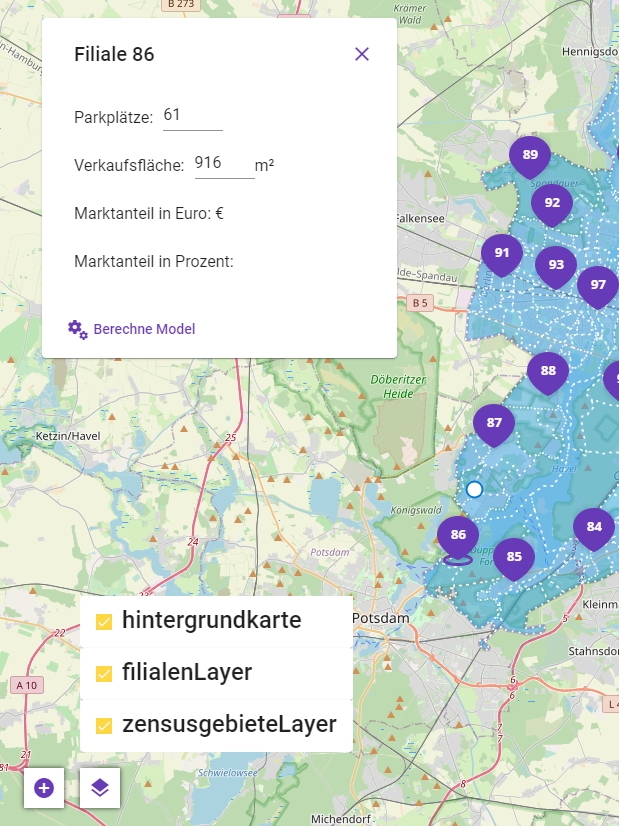
\includegraphics[scale=0.5]{resources/images/toolset.png}}
	\caption{Bildschirmausschnitt der UI-Elemente}
	\label{img:toolset}
\end{figure}

Bei der Umsetzung der UI-Elemente wurde auf die Komponenten-Bibliothek \emph{Angular Material} für fertige UI Komponenten zugegriffen \footcite{team_angular_material}.
Zu den benutzen Komponenten zählen Material Button \footcite{team_angular_material_button}, Icon \footcite{team_angular_material_icon}, Card \footcite{team_angular_material_card}, List \footcite{team_angular_material_list}, Input \footcite{team_angular_material_input} sowie Checkbox \footcite{team_angular_material_checkbox}.

Um eine bessere Visualisierung einzelner Featurelayer zu ermöglichen, sollen die Layer einzeln aus- beziehungsweise eingeblendet werden können.
Dies geschieht im Werkzeug Layermanager.
Hierzu müssen also innerhalb des Werkzeuges alle Layer angezeigt werden und über eine Checkbox die Sichtbarkeit verändert werden können.\\
Für die Konfiguration des Layermanagers werden zunächst über den BaseMap-Service alle Layer der Karte abgerufen.
Aus den Layer-Objekten werden nun Name- und Sichtbarkeit -Eigenschaften in jeweils ein neues LayerManagerEntry-Objekt extrahiert.
Im Layermanager können nun der Name und die Sichtbarkeit pro Layer dargestellt werden, wobei die Sichtbarkeit als Checkbox dargestellt wird.
Mit der Interaktion einer Checkbox wird über den zugehörigen Namen der entsprechende Layer im BaseMap-Service identifiziert und das \emph{Visible} Attribut angepasst.
Der Layermanager erscheint als Fenster nach Aktivierung des entsprechenden Knopfes (Icon: \emph{layer}, siehe Abbildung \ref{img:toolset}).

\begin{lstlisting}[language=JavaScript]
	
type LayerManagerEntry = { layerIdentifier: LayerIdentifier, visibility: boolean };

public layerManagerEntries: LayerManagerEntry[];

this.layerManagerEntries = baseMapService.getLayers().getArray().map(layer => {
	return {
		layerIdentifier: layer.get('name'),
		visibility: layer.getVisible()
	} as LayerManagerEntry;
});

setLayerVisibility(event: any, layerIdentifier: LayerIdentifier): void {
	if (event.checked) {
		//  show layer
		this.baseMapService.getLayers().getArray().find(layer => layer.get('name') === layerIdentifier).setVisible(true);
	} else {
		//  hide layer
		this.baseMapService.getLayers().getArray().find(layer => layer.get('name') === layerIdentifier).setVisible(false);
	}
}
\end{lstlisting}

Vervollständigt wird das Werkzeug-Set durch die Interaktion eine neue Filiale auf der Karte zu setzen.
OpenLayers bietet hierzu eine Draw-Interaktion, die es erlaubt einer Layersource ein neues Feature hinzuzufügen.

\begin{lstlisting}[language=JavaScript]

private addDrawInteraction(): void {
	this.drawInteraction = new Draw({
		type: GeometryType.POINT,
		source: this.tempFilialeLayer.getSource(),
		style: NEW_STORE_INTERACTION_STYLE
	});
	
	this.drawInteraction.on('drawend', (drawEndEvent) => {
		const feature = drawEndEvent.feature;
		
		// new feature needs an new ID or OL Fails with https://openlayers.org/en/v6.3.1/doc/errors/#30
		feature.setId(new Date().getTime());
		featureService.addFiliale(feature);
		this.deactivateAddFiliale();
	});
	this.baseMapService.addInteraction(this.drawInteraction);
}
\end{lstlisting}

In der Initialisierung der Interaktion wird festgelegt, dass nur Punkte erstellt werden können, sowie über einen \emph{NEW\_STORE\_INTERACTION\_STYLE} wird dem Punkt ein eigener Style zugewiesen (ersichtlich in Abbildung \ref{img:toolset}).
Ebenso wird ein temporärer Layer für die neu gesetzte Filiale für die Dauer der Interaktion definiert.
Da auf der neuen Filiale die Attribute Parkplätze und Verkaufsfläche, sowie die Attraktivität noch nicht gesetzt wurden, ist es einfacher für die Interaktionsdauer einen temporären Layer zu verwenden, der nach Interaktionsende das erstellte Feature an den Feature-Service übergibt, wo die fehlenden Attribute gesetzt werden und das Feature in den Filiallayer übertragen wird. 
Sobald die Interaktion der Karte hinzugefügt wurde, muss lediglich bei Aktivierung der temporäre Layer der Karte hinzugefügt werden, damit die Interaktion sichtbar ist.
Ebenso müssen andere Interaktionen, vor Allem die Feature-Selektierung der Filialen und Gebiete (Implementierung erfolgt im späteren Verlauf des Kapitels), deaktiviert werden, damit es hierbei nicht zu ungewollten, parallelen Interaktionsaufrufen kommt.
Sobald eine neue Filiale gesetzt wurde, muss der Layer wieder entfernt, die Interaktion deaktiviert und andere Interaktionen reaktiviert werden.
Aktiviert wird die Interaktion über den entsprechenden Knopf auf der Karte (Icon: \emph{add\_icon}, siehe Abbildung \ref{img:toolset}).

Für die Platzierung im DOM werden beide Werkzeuge in einer Werkzeug-Set Komponente zusammengefasst, die ein einheitliches Styling erlaubt.

Als nächstes muss das Objektfenster, welches bei Selektion eines Features geöffnet werden soll und wichtige Informationen über die Filiale oder das Gebiet enthält, implementiert und in den DOM gesetzt werden.\\
Das Objektfenster ist ein Fenster welches sich wie schon der Layermanager über die Karte legt und Informationen über ein ausgewähltes Feature bietet. 
Selektiert können sowohl Filialen als auch Zensusgebiete werden.
Im Falle einer Filiale soll das Objektfenster auch die Berechnung des Huff-Modells für diese Filiale ermöglichen.\\
Über einen Objektfenster-Service wird das momentan ausgewählte Feature in Form eines \emph{Obervables} \footcite{rxjs_observable} bereitgestellt und ist jederzeit abrufbar.
In Angular erfolgt dieser Aufruf über eine gesetzte \emph{Subscription} \footcite{rxjs_subscription} auf ein Observable.
In einer Angular Anwendung werden Komponenten über mehrere Lifecycle-Zyklen instanziiert, die eine besondere Datenübertragung innerhalb der Anwendung erfordern.
So erfolgt ein initiales Rendering des Templates und der Daten und Änderungen werden über eine \emph{ChangeDetection} erkannt und neu gerendert.
Um Fehler während des ChangeDetection-Lifecycles zu verhindern, erfolgt die Datenübertragung mit Obersvables \footcite{angular_lifecycle}.\\
Im Fall des Objektfensters subscribed die Komponente sich auf das \emph{currentlySelectedFeature\$} des Objektfenster-Services.
Dies bedeutet die Komponente erhält über ein Event direkt die neuesten Änderungen sobald sich das Observable ändert. 
Es erfolgt also kein expliziter, synchroner Datenaufruf, sondern das Observable sendet asynchron Änderungen an alle Subscriber.
Somit kann die Selektierung eines neuen Features problemlos an das Objektfenster weitergeleitet werden und die neuen Daten werden korrekt dargestellt. \\
Das Objektfenster für Filialen zeigt die folgenden Informationen:

\begin{itemize}
	\item Id
	\item Parkplätze
	\item Verkaufsfläche in Quadratmetern
	\item Marktanteil in Euro \footnote{\label{afterCalc}Nach Berechnung des Huff-Modells}
	\item Marktanteil in Prozent \cref{afterCalc}
\end{itemize}

Für ein Gebiet werden folgende Informationen angezeigt:

\begin{itemize}
	\item Id
	\item Einwohner
	\item Kaufkraft in Euro (Durchschnitt pro Monat pro Person)
	\item Ausgaben für Lebensmittel (Durchschnitt pro Monat pro Haushalt) 
	\item Wahrscheinlichkeitsfaktor (für den Besuch einer Filiale) \cref{afterCalc}
	\item Marktanteil der Filiale im Gebiet in Euro \cref{afterCalc}
	\item Marktanteil der Filiale im Gebiet in Prozent \cref{afterCalc}
\end{itemize}

Die Informationen zu Parkplätzen und Verkaufsfläche werden über ein Input-Feld dargestellt (siehe Abbildung \ref{img:filiale}).
Diese Parameter werden für die Attraktivitätsberechnung der Filiale verwendet und müssen für neue Filialen eingegeben werden.
Bei bestehenden Filialen lässt sich somit aber auch die Berechnung des Huff-Modells für die gleiche Filiale mit verschiedenen Parametern ermöglichen.

\begin{figure}[H]
	\makebox[\textwidth][c]{
		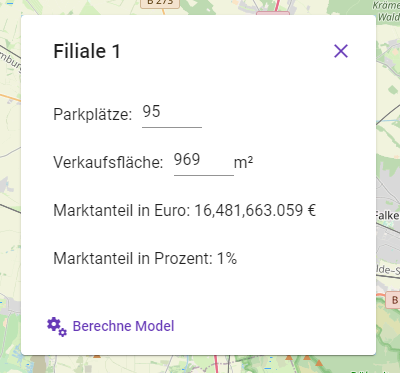
\includegraphics[scale=0.5]{resources/images/filiale_of.png}}
	\caption{Bildschirmausschnitt des Objektfensters einer Filiale}
	\label{img:filiale}
\end{figure}

Das Objektfenster öffnet sich automatisch nach dem Anlegen einer neuen Filiale.
Hierbei werden die Parkplätze und Verkaufsfläche zunächst mit jeweils dem Wert Null angelegt und angezeigt.
Bevor das Huff-Modell berechnet werden kann, müssen valide Werte in beide Felder eingetragen werden, da solange der Knopf deaktiviert ist.
Die Aktivierung des Knopfes erfolgt über die einfache Validierung der Werte auf eine positive Zahl.\\
Der Knopf zur Berechnung des Huff-Modells ruft eine Funktion im Feature-Service auf, die die Berechnung für die ausgewählte Filiale durchführen soll.
Über den Schließ-Knopf (Icon: \emph{close}, siehe Abbildung \ref{img:filiale}) wird das Objektfenster geschlossen und der Wert des Observables \emph{currentlySelectedFeature\$} auf \emph{null} gesetzt.

Mit der Implementierung des Objektfensters sind nun sämtliche Komponenten der Anwendung bereit, die für Berechnung des Huff-Modells und anschließenden farbliche Einfärbung der Zensusgebiete erforderlich sind.

Die Berechnung des Huff-Modells erfolgt im Feature Service.
Die für das Huff-Modell erforderliche Parameter Attraktivität und Faktor der Attraktivität $\alpha$, sowie Distanz und Faktor der Distanzfunktion $\beta$ müssen bestimmt werden.
Wie bereits im Kapitel \ref{subsec:gravitationmodel} zum Gravitationsmodell nach Huff erläutert, sind die Faktoren $\alpha$ und $\beta$ für die Berechnung im realen Wirtschaftsumfeld empirisch anhand von realen Markt- und Wirtschaftsdaten aus Umfragen mit Kunden zu analysieren und zu bestimmen.
Für den Prototypen sind diese Werte auf 1,5 für $\alpha$ und 1,5 für $\beta$ festgelegt.
Angenommen wird also, dass je attraktiver eine Filiale ist desto Wahrscheinlicher auch ein Besuch eines Kunden ist.
Ebenso, je näher ein Kunde an einer Filiale wohnt desto wahrscheinlicher ist auch hier der Besuch der Filiale.\\
Die Attraktivität A der Filiale wird über die Summe der Parkplätze und Verkaufsfläche berechnet.
Je größer eine Filiale desto größer ist wahrscheinlich das Sortiment und die Menge der Lebensmittel.
Und je mehr Parkplätze vor der Filiale vorhanden sind desto mehr Kunden können angezogen werden, die einen weiteren Anreiseweg haben oder mehr auf einmal einkaufen wollen.
Für die Berechnung der Attraktivität sind viele weitere Parameter denkbar jedoch bieten die Anzahl der Parkplätze und die Verkaufsfläche in Quadratmetern aus den aufgeführten Gründen eine fundierte Grundlage für die Bewertung der Attraktivität.\\
Die Distanz D der Filiale zu den Gebieten ist eine einfache Distanzberechnung in OpenLayers vom Standort der Filiale zum Mittelpunkt des jeweiligen Gebiets.
Zunächst werden aus den Features der Gebiete über \emph{Type Assertion} Multipolygone über die OpenLayers interne Funktionen zur Mittelpunktbestimmung bieten.
Da Multipolygone mehrere Mittelpunkte haben, wird der erste Eintrag aus dem Array gewählt.\\
OpenLayers bietet für die Längen- und Größenberechnung verschiedene Funktionen, die sich in der Berechnung unter Einbezug der Projektion unterscheiden \footcite{openlayers_measure_example}.
Die Koordinaten der Filiale und des Mittelpunkts des Gebiets werden zu einem \emph{LineString} Objekt zusammengefasst \footcite{openlayers_linestring}.
Von dieser Linie wird nun die Länge berechnet.
Wird die einfache Berechnung \emph{LineString.getLength()} verwendet, berechnet OpenLayers die Länge anhand von Orthodromen \footcite{orthodrome_frassek} oder der Großkreisdistanz \footcite{great_circle_distance}.
Wenn auch hervorragend für Flugdistanzen verwendbar, lässt diese Berechnung die Ergebnisse für Entfernungen auf dem Boden ungenau werden.\\
Über das \emph{Sphere} Paket von OpenLayers lässt sich aber eine Länge anhand der Projektion der Karte berechnen, welches zu den gewünschten Ergebnissen führt \footcite{openlayers_sphere}.

\begin{lstlisting}[language=JavaScript]
	
	// distance decay
	const DIST_DECAY = 1.5;
	// attractiveness enhancement factor
	const ATT_ENHANCE_FACTOR = 1.5;
	
	const centerCoordinates = (gebietFeature.getGeometry() as MultiPolygon).getInteriorPoints().getFirstCoordinate();
	
	const distance = ol_sphere.getLength(new LineString([filialCoordinates, centerCoordinates]), {projection: 'EPSG:3857'});
	
	const attractiveness = filiale.parkingSpaces + filiale.salesArea;
	
\end{lstlisting}

Über den Knopf \emph{Berechne Huff-Modell} (Icon: \emph{miscellaneous\_services}, siehe Abbildung \ref{img:filiale}) im Objektfenster der ausgewählten Filiale wird die Id der Filiale an den Feature Service übergeben und die Berechnung gestartet.
Über die Id wird das Feature der entsprechenden Filiale im Filiallayer identifiziert und kann bearbeitet werden.\\
Die Wahrscheinlichkeit des Besuchs eines Gebiets für die ausgewählte Filiale innerhalb des gesamten Filialnetzes ergibt sich, wenn die Wahrscheinlichkeit der ausgewählten Filiale ins Verhältnis zur Netzwahrscheinlichkeit gesetzt wird.
Für die Filiale errechnet sich die Wahrscheinlichkeit des Besuchs der einzelnen Gebiete daher anhand von zwei \emph{ForEach} Schleifen.
Zunächst wird über alle Gebiete iteriert, um die Wahrscheinlichkeit sämtlicher Gebiete für die ausgewählte Filiale zu berechnen.
In der Schleife der Gebiete muss für jedes Gebiet über die Filialen iteriert werden, um die Menge der Wahrscheinlichkeiten aller Filialen zu dem Gebiet zu berechnen.

\begin{lstlisting}[language=JavaScript]
	
	zensusgebiete.forEach(gebiet => {
		// probability for all stores
		let netProbability = 0;
		
		// probability for the selected store alone
		const storeProbability = Math.pow(filiale.attractiveness, this.ATT_ENHANCE_FACTOR) / Math.pow(distance, this.DIST_DECAY);
		
		filialen.forEach(store => {
			netProbability += Math.pow(store.attractiveness, this.ATT_ENHANCE_FACTOR) / Math.pow(this.calculateDistancesForFiliale(store.coordinates, gebiet.coordinates), this.DIST_DECAY);
		});
	
		// probability inside net of stores
		gebiet.probability = storeProbability / netProbability;

		// marketshare
		gebiet.marketShare = gebiet.spendituteGroc * gebiet.probability;
		gebiet.marketSharePercentage = gebiet.marketShare / gebiet.spendituteGroc;
	});
\end{lstlisting}

Nachdem jedes Gebiet Besuchswahrscheinlichkeiten ausgerechnet bekommen hat, wird der Marktanteil prozentual sowie monetär für ein besseres Verständnis sowie eine bessere Einordnung errechnet.
Hierzu werden die Ausgaben des Gebiets für Lebensmittel im Monat mit der Wahrscheinlichkeit des Besuchs multipliziert, um den Anteil der Lebensmittelausgaben in Euro des Gebiets für die ausgewählte Filiale zu errechnen.
Wird dieser Betrag nun ins Verhältnis zu den Gesamtausgaben für Lebensmittel im Gebiet gesetzt, errechnet sich der prozentuale Anteil.
Erfolgten diese Schritte für alle Gebiete und werden die Beträge des Anteils der Ausgaben der Filiale und der Gesamtausgaben pro Gebiet summiert, ergibt sich der Marktanteil der Filiale im Netz in Euro und, im Verhältnis zu einander, in Prozent.

\begin{lstlisting}[language=JavaScript]
	
	let marketShareTotal = 0;
	let totalMarketExpenditure = 0;
	this._zensusMap.forEach((gebiet: ZensusProperties) => {
		marketShareTotal += gebiet.marketShare;
		totalMarketExpenditure += gebiet.spendituteGroc;
	});
	filiale.marketShare = marketShareTotal;
	filiale.marketSharePercentage = marketShareTotal / totalMarketExpenditure;
	
\end{lstlisting}

Bei jeder Berechnung der Wahrscheinlichkeit des Besuchs der Gebiete für die ausgewählte Filiale wird final nun noch das Gebiet eingefärbt.
Hierzu wird auf jedem abhängig der errechneten Wahrscheinlichkeit ein Indikator gesetzt, der einer bestimmten Farbe entspricht.

\begin{lstlisting}[language=JavaScript]
	
	const probabilityInPercent = gebiet.probability * 100;
	
	if (probabilityInPercent > 80) {
		gebiet.indicator = 1;
	}
	else if (probabilityInPercent < 80 && probabilityInPercent > 70) {
		gebiet.indicator = 2;
	}

	...
	
	else {
		gebiet.indicator = 9;
	}
\end{lstlisting}


Dieser Indikator wird im Renderzyklus der Gebiete innerhalb der \emph{StyleFunction} pro Gebiet ausgelesen und das Gebiet entsprechend eingefärbt (ähnlich zur StyleFunction der Filialen \ref{code:filialStyle}).

\begin{lstlisting}[language=JavaScript]
	
	protected readonly colorGradient: ColorInterface[] = [
	{ gravitationalRing: 1, value: 'rgb(255,100,100)'},
	{ gravitationalRing: 2, value: 'rgb(252,145,145)'},
	{ gravitationalRing: 3, value: 'rgb(248,161,123)'},
	{ gravitationalRing: 4, value: 'rgb(232,180,112)'},
	{ gravitationalRing: 5, value: 'rgb(208,198,117)'},
	{ gravitationalRing: 6, value: 'rgb(178,214,138)'},
	{ gravitationalRing: 7, value: 'rgb(138,217,157)'},
	{ gravitationalRing: 8, value: 'rgb(90,217,183)'},
	{ gravitationalRing: 9, value: 'rgb(0,215,212)'}
	];
	
	const gebieteStyle = new Style({
		stroke: new Stroke({
			color: 'white',
			width: 2,
			lineDash: [0.1, 7]
		}),
		fill: new Fill({
			color: 'rgba(52, 164, 235, 0.5)'
		})
	});

	const gebieteStyleFunction = (feature, resolution) => {
		const indicator = feature.indicator;
		
		if (!indicator) {
			return this.ezbLineStyle;
		}
		const color = colorGradient.find(color => color.gravitationalRing === indicator).value;
		gebieteStyle.getFill().setColor(color);
		return gebieteStyle;
	}
\end{lstlisting}
